\chapter{God gave us numbers, and human thought created algorithms}
\label{chap:sets_and_numbers}

\begin{figure}[ht]
\begin{center}
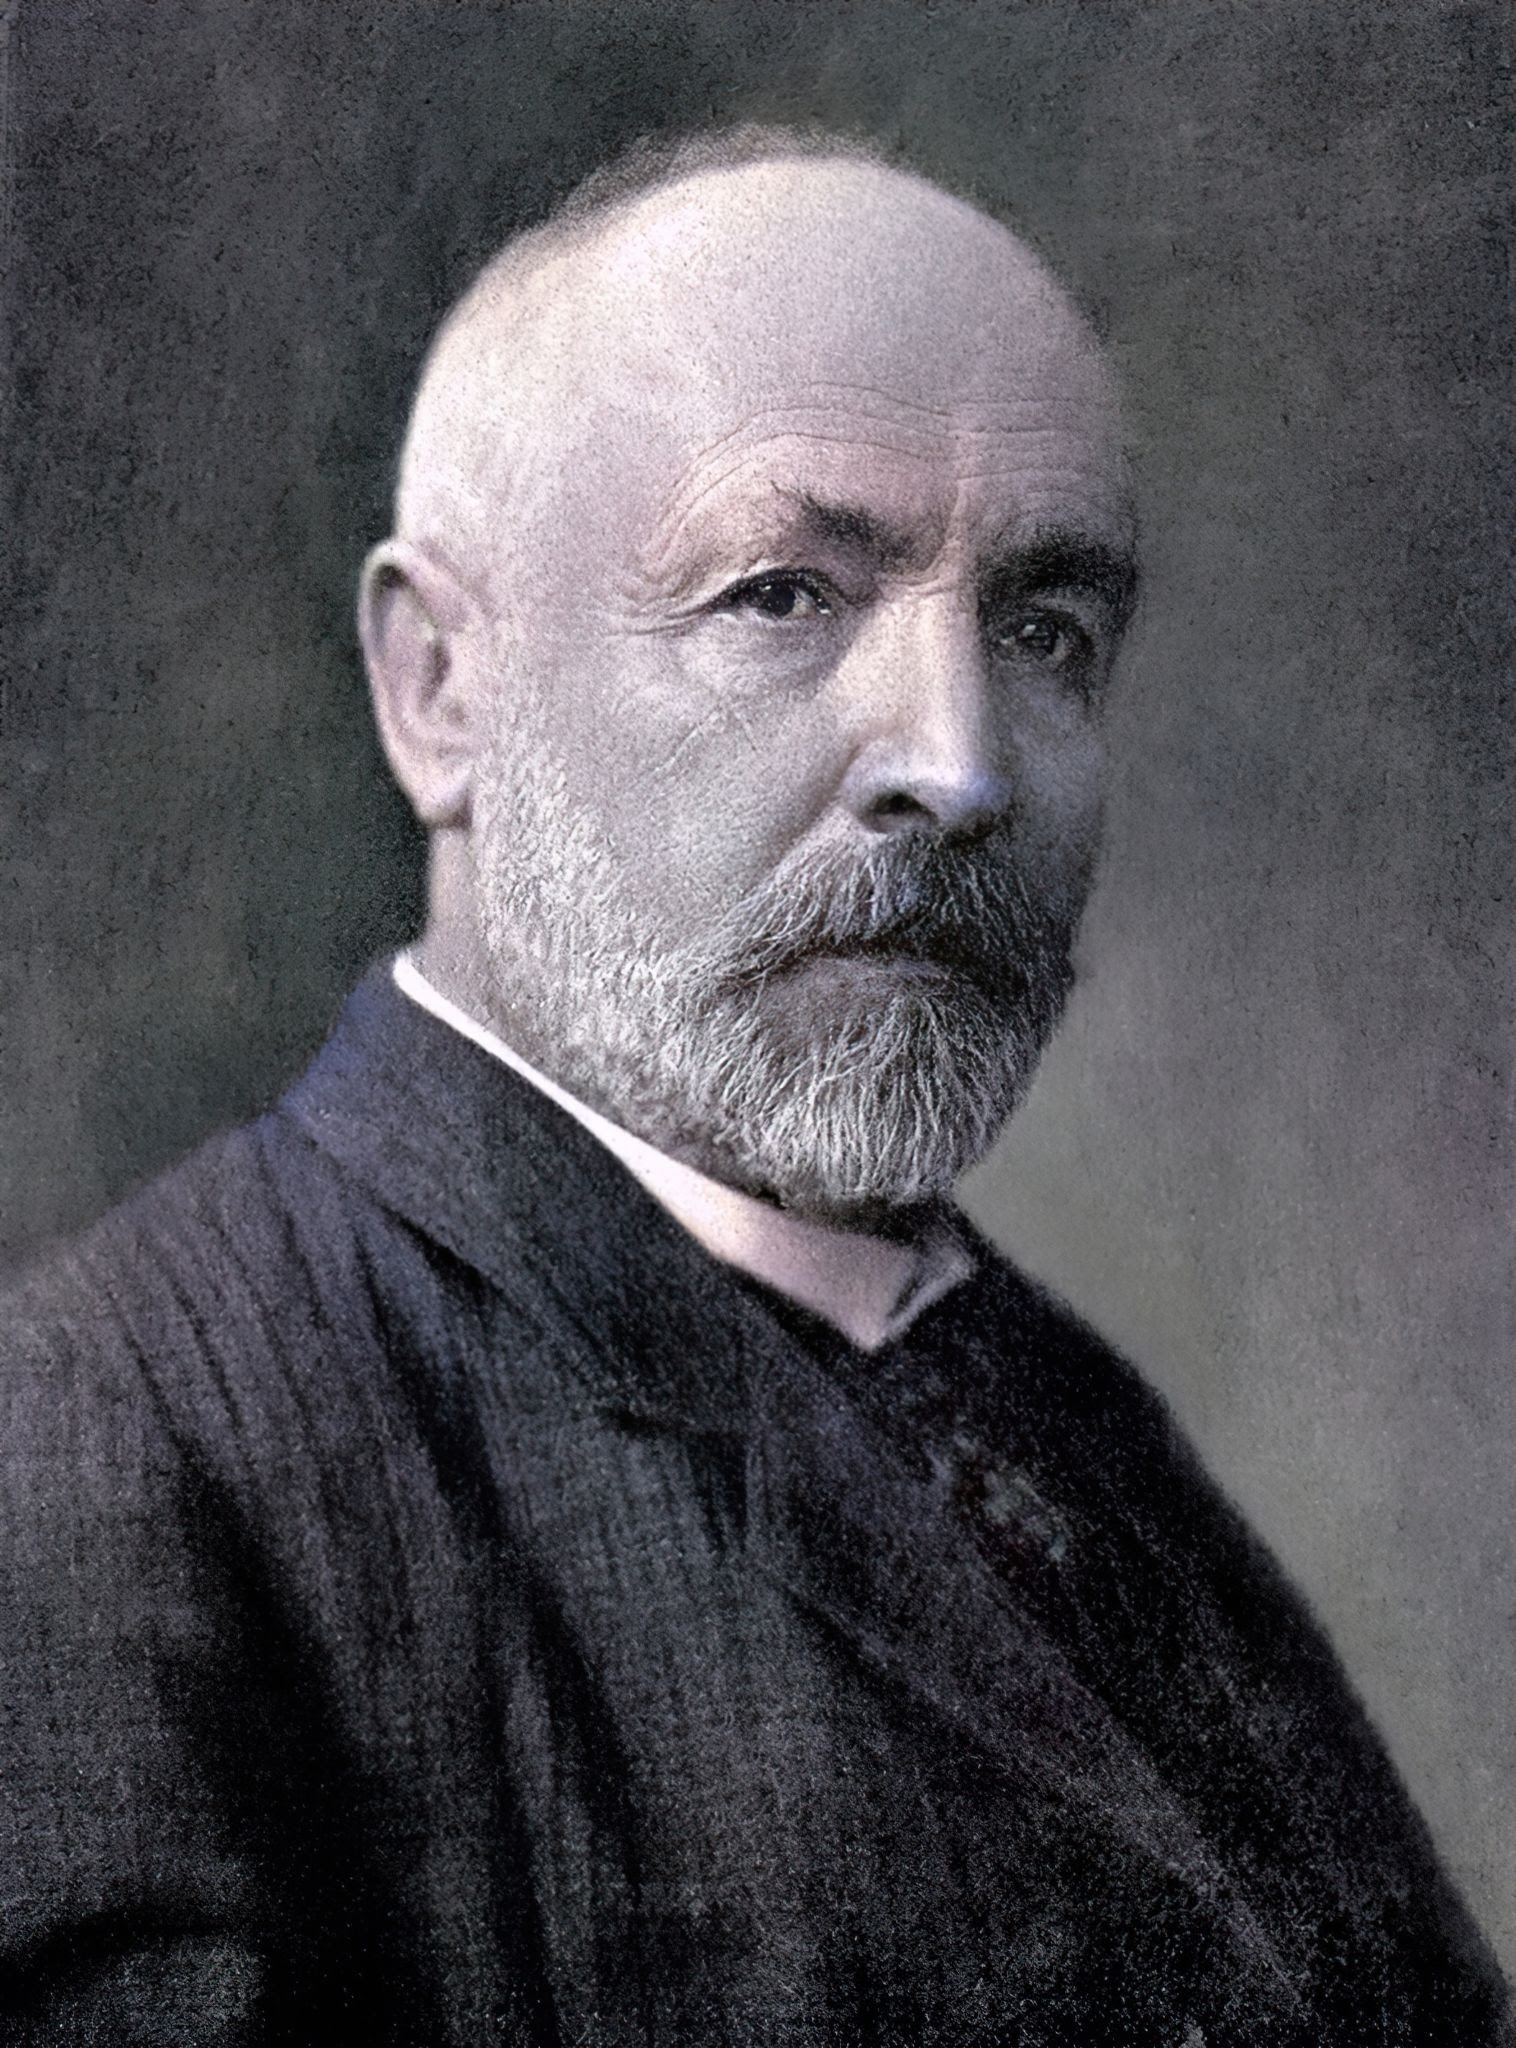
\includegraphics[width=1.0in]{images/cantor.jpeg}

\caption*{\small ``In mathematics the art of proposing a question must be held of higher value than solving it.'' \\
``A set is a Many that allows itself to be thought of as a One.''   -- Georg Cantor}
\end{center}
\end{figure}


\begin{figure}[ht]
\begin{center}
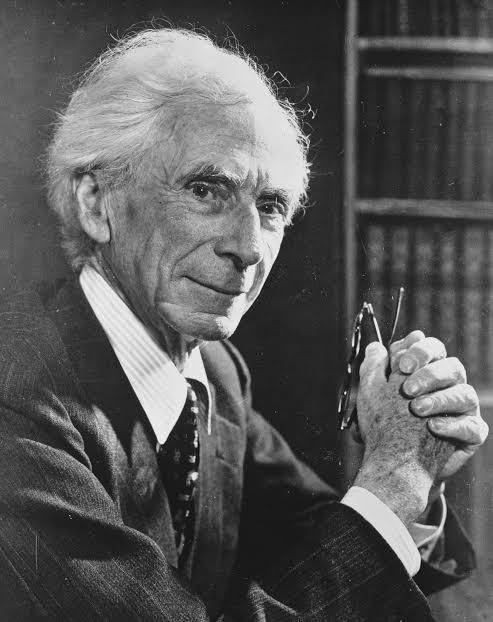
\includegraphics[width=1.0in]{images/russell.jpeg}
\caption*{\small ``A number will be a set of classes such as that any two are similar to each other,  and none outside the set are similar to any inside the set.'' \\
                ``Mathematics rightly viewed possesses not only truth but supreme beauty.'' -- Bertrand Russel}
\end{center}
\end{figure}

\section{Numbers}
\label{sec:numbers}
Our discussion on mathematics and computing must start with numbers. What are numbers after all? The same number may be represented  with symbols such as 3,  III, or even as a line of a fixed length. But what is the underlying concept behind the different representations?

\href{https://en.wikipedia.org/wiki/Bertrand_Russell}{Bertrand Russell} defined numbers as sizes (or {\em cardinality}) of {\em collections}. Some examples of  {\em equinumerous} collections are $\{Red, Blue, Green\}$, $\{Amir, Salman, Shahrukh\}$, $\{Godavari, Kaveri, Krishna\}$. {\em Collections} are also called {\em Sets} or {\em Classes} in Mathematics. All three Sets above are of cardinality 3. Russel defined a number as -- {\em the number of a class is the class of all those classes that are similar (equinumerous) to it}. So, according to Russel, a number is a class of classes.  

Note that {\em cardinality} of sets is not the only way to describe the concept of a number. A number may also be a measure of a length. For example, in the straight line below, if we define the segment $\overline{0a}$ to be the {\em unit length} representing the number 1, then the line segment $\overline{0b}$ which is twice the length of $\overline{0a}$ may  represent the number 2.

\vspace{0.5in}
\begin{tikzpicture}[stop jumping,constrain]
\path(0,0) node[name=O,ruler compass/point=red,label={0}];
\path (O)++(0:2) node[ruler compass/point=red,label={a}];
\ruler{O}{a}
\path (a)++(0:2) node[ruler compass/point=red,label={b}];
\ruler{a}{b}
%\compass{O}{a}
\end{tikzpicture}
\vspace{0.5in}

Without belabouring the point, it will suffice to say for our purpose that all of us intuitively understand what numbers mean.

\subsection{Numbers may be represented in multiple ways}

However, we need to do useful stuff with numbers -- we need to add, subtract, multiply and divide them for obvious practical reasons.  Indeed, the history of numbers date back to the Mesolithic stone age. The early humans had to figure out -- due to a variety of practical considerations -- that if they put two similar collections of size two and size three together, the larger collection becomes of size five.  

Civilisations have found many ways to represent numbers through the ages. Some examples are as tally marks in the prehistoric to early civilisations  -- as straight marks on bones, sticks, or stones --  as can be observed in the archaeological evidence of the Ishango bones from around 20000 BCE; as Egyptian --  a stroke for 1, heel bone for 10, coil of rope for 100, etc. -- or Roman -- I, V, X, L, C, D, M -- numerals; as Base-60 (sexagesimal) numbers written as combinations of ``1'' and ``10'' wedges by the Babylonians around 2000 BCE; as used rods arranged on counting boards in base-10 with positional notation in Chinese rod systems;  as positional decimal systems in Indian numerals in the Gupta period around $5^{th}$ century CE;  as beads or stones moved on rods or grooves to represent numbers in Abacus systems in China, Rome, Mesopotamia and Jerusalem; with  Indo-Arabic numerals in the medieval period; with various mechanical calculators such as  Napier’s bones,  Slide rules,  Pascal’s calculator, and  Leibniz's stepped reckoner in the $17^{th}$ century; as gears and levers in Charles Babbage's first programmable computer -- the Analytic Engine; and as bits and bytes in modern digital computers. Note, also, that the methods of carrying out these operations -- the algorithms -- will necessarily depend on the representation we choose for numbers. 

\section{Sets}
\label{sec:sets}
We will use {\em Sets} quite a bit in this course. We may describe a {\em Set} or a {\em Collection} by explicitly listing out its elements without duplicates, such as in the examples above. We may sometimes also describe a Set with a property like ``all students enrolled in the QRMT section FC-0306-3". We write this formally using a variable $x$ as $\{x \mid \mbox{$x$ is a student in the QRMT section FC-0306-3}\}$. The symbol $\mid$ is read as ``such that". 

If an element $x$ belongs to a set $A$, we usually write this as $x \in A$.

Here are some more examples of Sets:
\begin{enumerate}
\item $A = \{x \mid \mbox{$x$ is a student pursuing a degree in India}\}$
\item $B = \{x \mid  \mbox{$x$ is a CS Major student at Ashoka University}\}$
\item $C = \{x \mid \mbox{$x$ is a CS Major student at Ashoka University {\bf and} $x$ is female}\}$
\end{enumerate}

Clearly, all members of $C$ are also members of $B$, and all members of $B$ are members of $A$. We then say that $C$ is a {\em subset} of $B$  ($C \subseteq B$), and  $B$ is a {\em subset} of $A$ ($B \subseteq A$).  Formally, a set $B$ is a {\em subset} of another set $A$, denoted as $B \subseteq A$, if
$x \in A$ whenever $x \in B$. The empty set is denoted by $\phi$, its size is zero (0), and it is a subset of all sets.


Given two sets $A$ and $B$, the {\em union} $A \cup B$ is the set of all elements that are in $A$, or in $B$, or in both. Formally, $A \cup B = \{ x \mid x \in A \; \text{or} \; x \in B \}$. For example, if $A = \{1, 2, 3\}$ and $B = \{3, 4, 5\}$, then  $A \cup B = \{1, 2, 3, 4, 5\}$.

Given two sets $A$ and $B$, the {\em intersection} $A \cap B$ is the set of all elements that are in both  $A$ and $B$. Formally, 
$A \cap B = \{ x \mid x \in A \; \text{and} \; x \in B \}$. For example, if  $A = \{1, 2, 3\}$ and  $B = \{3, 4, 5\}$, then  $A \cap B = \{3\}$.

Clearly, for any set $A$, $A \cup \phi = A$ and $A \cap \phi = \phi$,

\begin{exercise}
Suppose $B \subseteq A$. Argue that
\begin{enumerate}
\item $A \cup B = A$
\item $A \cap B = B$
\end{enumerate}
\end{exercise}

\section{The set of Natural numbers}

Some sets can also be unbounded or infinite. We define the set of {\em Natural numbers} as $\N = \{0,1,2,3,\ldots\}$\footnote{0 is usually not included in the Set of Natural numbers in Mathematics. We will however include 0 in the set of Natural numbers in this course. After all,  it is quite natural to score a 0 in an examination}. 

While we all intuitively  understand this set, note that the elements of the set are as yet uninterpreted and undefined. We can overcome this lacunae by assuming a {\em God-gifted} ability to count. Given a number $n$ as the size of a Set or a length, let us assume that we can interpret and construct the successor of $n$ as $S(n) = n+1$. Then, we can formally define the set of Natural numbers $\N$ as:

\begin{definition}[Natural numbers]
~ \newline
\begin{enumerate}
\item $0 \in \N$, where $0$ is the symbol that denotes the size of the empty set, and
\item if $n \in \N$,  then $S(n) = n+1 \in \N$
\end{enumerate}
\end{definition}

We can then adopt a suitable representation for  successive elements in the set $\N$. Note that the set $\N$ is unbounded, because every number -- no matter how large -- has a successor.

The natural numbers are the numbers that we use for counting. Their usual order
begins
\[
0<1<2<3<\cdots.
\]
Thus there is a first natural number, and every natural number has a successor.
There is another important feature of this ordering: whenever we select a
non-empty collection of natural numbers, that collection has a smallest member.
This observation is called the \emph{Well-Ordering Principle}.

\subsection{The Well-Ordering Principle}
\label{sec:well-ordering}
Formally, the Well-Ordering Principle states that every non-empty subset of
$\N$ has a least element. That is, if $A\subseteq\N$ and $A\neq\phi$, then
there is an $m\in A$ such that
\[
m\leq a\qquad\mbox{for every }a\in A.
\]
For example, the set $\{5,8,11,14,\ldots\}$ has least element $5$. Similarly,
if
\[
A=\{n\in\N\mid n^2>1000\},
\]
then $30^2=900$, $31^2=961$, and $32^2=1024$, so the least element of $A$
is $32$.

This property is special to the natural numbers with their usual ordering. 

The Well-Ordering Principle makes precise an idea that is already present in
counting. If some natural numbers have a particular property, then there is a
\emph{first} natural number having that property. This also gives a useful way
of reasoning about a claim $P(n)$ that is supposed to hold for every
$n\in\N$. If the claim were false, the set
\[
C=\{n\in\N\mid P(n)\mbox{ is false}\}
\]
would be non-empty and would therefore have a least element. This element would
be the \emph{smallest counterexample}. Since every smaller natural number would
satisfy $P$, one can often use that fact to show that the smallest
counterexample must also satisfy $P$, obtaining a contradiction.

This method foreshadows the Principle of Mathematical Induction. In fact, the
Well-Ordering Principle for $\N$ and the Principle of Mathematical Induction
are equivalent: each can be used to prove the other. We shall return to this
connection when we study methods of proof.\footnote{ The Well-Ordering Principle used here should not be confused with the much more
general \emph{Well-Ordering Theorem}, which states that every set can be supplied
with some well-ordering. The Well-Ordering Theorem is equivalent to the Axiom of
Choice. Neither that theorem nor the Axiom of Choice is required for our present
discussion of $\N$.}

\subsection{Addition}

We observed that the underlying concept of a number is independent of specific representations. Ideally, so should be the concepts of carrying out various operations with numbers. We may think of addition -- the sum $a+b$ of two numbers $a$ and $b$ -- as just combining two similar sets of sizes $a$ and $b$. However, the procedure for ``combining'' is not representation independent. While simple ``putting together'' may work if we represent the numbers as collections of stones or marbles, it is not well defined for adding two numbers in the place-value representation that we are familiar with from junior school. Hence ``combining'' is a somewhat unsatisfactory way of defining addition. 

A better way of defining $a+b$ is by using the successor operation $S(a) = a+1$, $b$ times.  As long as we have a primitive method for computing $a+1$ in any representation for an arbitrary $a$, this definition of $a+b$ becomes representation independent.  We may  define the basic property of addition  using counting as:

For all $m,n \in \N$:
\begin{enumerate}
\item $m + 0 = m$
\item $m + S(n) = S(m+n)$
\end{enumerate}

In the above definition we have used the same trick as in definition of the set $\N$ above, of defining a larger concept as a successor of a smaller concept.  The process repeats, and the actual additions happen in the return path. For example,

\begin{eqnarray*}
\lefteqn{7+5}\\
 & & = (7 + 4) + 1\\
 & & = ((7 + 3) + 1) + 1 \\
 & & = (((7 + 2) + 1)  + 1) + 1 \\
 & & =  ((((7 + 1) + 1)  + 1) + 1) + 1\\
 & & =  (((((7 + 0) + 1) + 1) + 1)  + 1)  + 1 \\
 & & =  ((((7 + 1)  + 1) + 1) + 1) + 1\\
 & & =  (((8 + 1) + 1) + 1) + 1\\
 & & =   ((9 + 1)  + 1) + 1\\
 & & =   (10 + 1) + 1 \\
 & & =  11 + 1 \\
 & & = 12
\end{eqnarray*}

Note that the repeated substitution of a larger problem with a smaller problem is bounded, because the first condition of the definition works as a sentinel that we are bound to encounter as we keep reducing $n$.

We  can then describe a procedure for computing $a+b$ (Algorithm \ref{algo:sum}) based on the above principle, but avoiding the deferred computations. The procedure takes $a$ and $b$ as input and returns $sum$ as the output. $sum \leftarrow sum+1$ denotes the operation ``$sum$ is {\em assigned} $sum+1$'' indicating that $sum$ is incremented by 1.

\begin{algorithm}

\begin{algorithmic}[1]
\Procedure{add}{$a,b$}
\State $counter \leftarrow 0$
\State $sum \leftarrow a$  
\While{$counter < b$}
	\State $sum \leftarrow sum + 1$
	\State $counter \leftarrow counter + 1$
\EndWhile
\Return $sum$
\EndProcedure
\end{algorithmic}
\caption{An algorithm for $a+b$ by  $+1$ $b$-times. }
\label{algo:sum}
\end{algorithm}

\begin{exercise}
\begin{enumerate}
\item Assuming that the operation $a + 1$ is available as a primitive, convince yourself that the above procedure for adding two numbers are correct.
\item Argue that if the operation $a + 1$ is available as a primitive, then the above algorithm for addition is representation independent.
\item Describe how the algorithm may be implemented using pebbles or marbles to represent numbers.
\end{enumerate}
\end{exercise}

\subsection{Multiplication}
We can now define multiplication as repeated additions:

\begin{enumerate}
\item $n \times 0 = 0$, for all $n \in \N$
\item $n \times S(m) = n \times m + n$, for all $n,m \in \N$
\end{enumerate}
Note that here again we have defined $n \times S(m)$, in terms of a smaller problem $m \times n$ of the same type.
\begin{exercise}
\begin{enumerate}
\item Convince yourself that according to the above definition $n \times m = \underbrace{n + n + n + \ldots + n}_{m\; \; \mbox{times}}$.
\item Provide a representation independent algorithm, using only the successor function and addition, for multiplication of two numbers.
\item Describe how the algorithm may be implemented using pebbles or marbles to represent numbers.
\end{enumerate}
\end{exercise}

\subsection{Subtraction}

To define the subtraction operation $m-n$, we may first define a predecessor operation $P(n)$ -- analogous to $S(n)$  -- as
\begin{enumerate}
\item $P(0)$ is undefined
\item $P(n) = n - 1$ for all $n > 0$.
\end{enumerate}
We assume, as before, that we have a primitive counting based procedure for computing $P(n) = n - 1$ in any representation. We can define the subtraction operation $m - n$ similarly to addition:

For all $m,n \in \N, m \geq n$
\begin{enumerate}
\item $m - m = 0$
\item $m - n = S(P(m) - n)$
\end{enumerate}
As before, note that $P(m)-n$ is a smaller problem that $m-n$.

The subtraction algorithm may then be given as:


\begin{algorithm}
\begin{algorithmic}[1]
\Procedure{subtract}{$a,b$}
\State $counter \leftarrow 0$
\While{$counter < b$}
	\State $a \leftarrow  a - 1$
	\State $counter \leftarrow counter + 1$
\EndWhile
\Return $a$
\EndProcedure
\end{algorithmic}
\caption{An algorithm for $a-b$, $a \geq b$ by  $-1$ $b$-times. }
\label{algo:sub}
\end{algorithm}

\begin{exercise}
Provide alternative versions of Algorithms \ref{algo:sum} and \ref{algo:sub} without using the $counter$. Instead decrement $b$ using $b \leftarrow b-1$ repeatedly till $b = 0$.
\end{exercise}

\subsection{Division}

Division is a natural requirement in civilised societies, mainly for sharing. However, it may not always be possible to divide natural numbers in equal proportions. For example, a collection of size 3 cannot be divided in two proportions of equal sizes without breaking up at least one member element. We have the {\em division theorem}:
\begin{theorem}
Given two numbers $a,b \in \N$, there exist unique $q,r \in \N$ (quotient and remainder, respectively)  such that $a = bq + r$ and $0 \leq r < b$. 
\end{theorem}
\begin{proof}
Let us first argue that such $q$ and $r$ exist. Repeatedly compute $a - b,a - 2b, a - 3b, \ldots, a - kb$, $k \geq 0$, till $a - kb  <  b$ and subtraction is possible no more.  Set $q = k$ and $r = a -kb$. Clearly, $q$ is the total number of times $b$ can be subtracted from $a$, and $0 \leq r < b$. If $r=0$ then $b$ divides $a$ exactly.

To argue that that $q$ and $r$ obtained by the above procedure are unique, let us suppose they are not. Then, there exist $q_1,r_1$ and $q_2,r_2$ such that
\[
\begin{array}{l}
a = bq_1 + r_1, 0 \leq r_1 < 0 \\
a = bq_2 + r_2, 0 \leq r_2 < 0 
\end{array}
\]

Without loss of generality, let us assume that  $q_1 \geq q2$. The above implies that $b(q_1 - q_2) = r_2 - r_1$. One of two cases arise:
\begin{enumerate}
\item $q_1 = q_2$. This implies that $r_1 = r_2$, and hence uniqueness.
\item $q_1 > q_2$. This implies that $q_1 - q_2 \geq 1 \in \N$. Hence $r_2 - r_1 \geq b$. But this is not possible because $0 \leq r_1,r_2 < b$. Hence $q$ and $r$ must be unique.
\end{enumerate}
\end{proof}

In the above proof, we used {\em explicit construction} as a proof technique for establishing existence of such $q$ and $r$, and {\em contradiction} for establishing their uniqueness.  We will revisit these techniques later in the course when we discuss proofs.

\begin{exercise}
Describe an algorithm using repeated subtraction that computes $q$ and $r$ given $a$ and $b$.
\end{exercise}

\section{The Set of Integers}
\label{sec:int}
 
We defined  the subtraction operation $m-n, m \geq n, m,n \in \N$ as the number of times the successor operation $S()$ needs to be applied to reach $m$ from $n$. This definition requires the restriction that $m \geq n$. An obvious generalisation is to remove the restriction and measure the difference in terms of either the successor $S()$ or the predecessor $P()$ operator. Subtraction then becomes directional, and we require negative numbers to represent the direction. This leads us to the set of integers
\[
\Z = \{\ldots, -3,-2,-1,0,1,2,\ldots\}
\]

Arithmetic in the set $\Z$ follows the same principles as in $\N$, except that they are now directional.
\begin{exercise}
Rework the definitions and the algorithms for addition, multiplication, subtraction and division in $\Z$.
\end{exercise}

Note, that the set of negative integers
\[
\{-1,-2,-3,\ldots\}
\]
has no least element: given any member, there is always a smaller one. So, the set of  integers is not {\em well-ordered}.

\section{The Set of Rationals}
\label{sec:rat}
The division theorem tells us that given $m,n \in \N$, there exist $q,r \in \N$, such that $m$ can be divided in to $q$ parts of size $n$, possibly leaving a remainder $0 \leq r < n$. Division is an obvious fundamental need for resource sharing. If each unit is indivisible -- like live cattle, for example --  then the division theorem is the best we can do. However, items measured in units such as weight, volume or length --  such as meat from a hunted animal, or a pile of grains -- are often divisible in smaller proportions like $1/3^{rd}$, $2/25^{th}$ etc.  So, division inevitably leads us to fractions. We define the set of Rational numbers as
\[
\Q = \{x | x = p/q, p \in \Z, q \in \N, q \neq 0\}
\]
We often also write this as $\frac{p}{q}$. These are numbers of the type $\pm 1/1,\pm 1/2,\pm 1/3,\pm 1/4, \pm 2/5$ etc.  We may also insist that $p$ and $q$ should have no common factors (i.e., $gcd(p,q) = 1$;  see Section \ref{sec:gcd} for a formal definition of $gcd$) to avoid multiple representations for the same Rational number. Clearly $\N \subset \Z \subset \Q$.  

Note, however, that we now have a situation where between any two rational numbers there are infinitely many other rational numbers.
\begin{exercise}
Convince yourself of the above statement.
\end{exercise}

This implies that there is no well defined successor function for a rational number, and we need to revisit our definition of addition for rationals. We start by noting that, for example,
\[
\frac{1}{3} + \frac{2}{3} = \frac{1+2}{3} = 1
\]
i.e., we can add the numerators as in $\Z$ if the denominators are the same. However, the addition 
\[
\frac{2}{3} + \frac{3}{4}
\]
is not well defined unless the two fractions can be expressed in the same unit. But we can multiply the numerator and denominator of the first fraction by 4, and the second by three to convert to the same unit where the denominator of both is 12
\[
\frac{2 \times 4}{3 \times 4} + \frac{3 \times 3}{4 \times 3} = \frac{8}{12} + \frac{9}{12} = \frac{8+9}{12} = \frac{17}{12}
\]
Note that multiplying the numerator and the denominator of a fraction with the same number does not change the fraction. So, we can define the general rule for addition of two rational numbers as 
\[
\frac{p_1}{q_1} + \frac{p_2}{q_2} = \frac{p_1 \times q_2 + p_2 \times q_1}{q_1 \times q_2}
\]
where all the additions and multiplications are defined on the set $\Z$.

\begin{exercise}
Extend the above idea to define subtraction, multiplication and division in the set $\Q$.
\end{exercise}

 The set
of positive rational numbers
\[
\left\{1,\frac{1}{2},\frac{1}{3},\frac{1}{4},\ldots\right\}
\]
also has no least element, since $1/(n+1)<1/n$ for every positive natural
number $n$. Thus not every set of numbers is well-ordered by its usual order.

\section*{Problems}

\begin{enumerate}
  %\setcounter{enumi}{8}

  \item Give three different representations for the number 6 (for example: tally marks, Roman numerals, line segment lengths). Explain how the operation ``+1'' is carried out in each representation.  

  \item Research and briefly describe how numbers were represented in one historical number system not discussed in class (e.g., Mayan or Incan). Compare it with the decimal positional system.

  \item Let 
  \[
    A = \{x \mid x \text{ is an even number less than 20}\}, \quad 
    B = \{x \mid x \text{ is a prime number less than 20}\}.
  \]
  Compute $A \cap B$, $A \cup B$, and $A \setminus B$.

  \item Prove or disprove: If $A \subseteq B$ and $B \subseteq C$, then $A \subseteq C$.

  \item Construct a real-world example of three sets $A, B, C$ such that $C \subset B \subset A$.

  \item Using only the successor function $S(n) = n+1$, show step by step how to compute $4 + 3$.

  \item Show that addition defined by the recursive rules in the text is associative, i.e. prove $(a+b)+c = a+(b+c)$ using the definition.

  \item Starting from the definition $n \times S(m) = (n \times m) + n$, compute $3 \times 4$ step by step.

  \item Write pseudocode (representation-independent) for multiplication using only the successor function and addition.

  \item Explain how you could simulate multiplication using only pebbles to represent numbers.

  \item Using the predecessor function $P(n)$, compute $7 - 4$ step by step as in the recursive definition.

  \item Implement Algorithm 2 (subtraction by repeated decrementing of $b$) on the input $a = 10, b = 6$. Show the intermediate steps.

  \item Using the Division Theorem, compute the quotient and remainder when $a = 29, b = 5$ using repeated subtraction.

  \item Prove that the quotient and remainder obtained from the Division Theorem are unique.

  \item Extend the recursive definition of addition from natural numbers to integers, and compute $(-3) + 5$.

  \item Explain why we need negative numbers to generalize subtraction. Give a real-world example where negative numbers are essential.

  \item Give an example of two distinct rational numbers between $\tfrac{1}{3}$ and $\tfrac{1}{2}$.

  \item Prove that between any two rational numbers there exists another rational number. (Hint: use their average.)

  \item Compute $\tfrac{2}{3} + \tfrac{4}{5}$ using the common-denominator method.

  \item Extend the definition to show how to compute $\tfrac{3}{7} \div \tfrac{2}{5}$.

\end{enumerate}


\chapter{Ruler and compass algorithms}
\label{sec:rulerandcompasqs}
%

\begin{figure}[ht]
\begin{center}
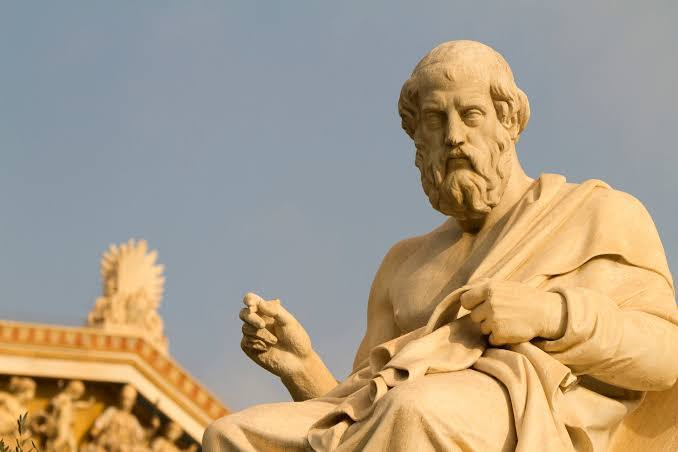
\includegraphics[width=1.5in]{images/plato.jpeg}
\caption*{\small ``Geometry is knowledge of the eternally existent… it compels the soul to look upwards, and leads us away from the world of appearance to the vision of truth.'' \\ ``Let no one ignorant of geometry enter here'' -- Plato}
\end{center}
\end{figure}


\begin{figure}[ht]
\centerline{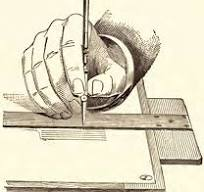
\includegraphics[width=2.0in]{images/straight.jpg}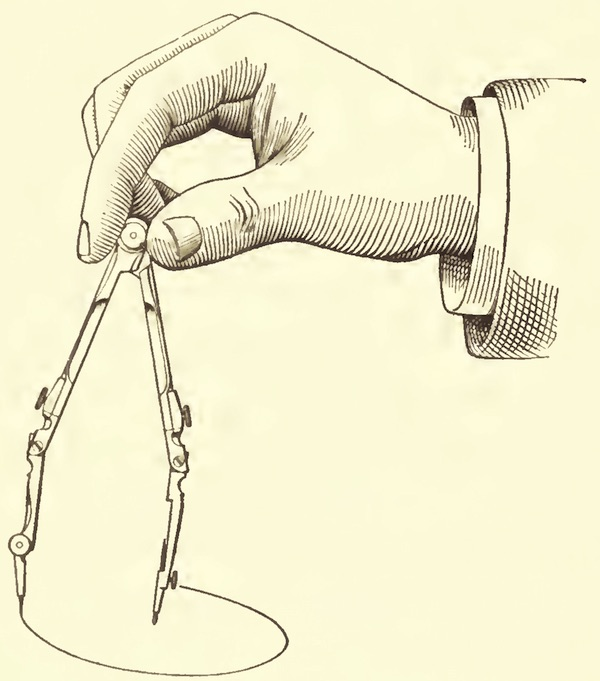
\includegraphics[width=2.0in]{images/compass.jpg}}
\caption{Ruler and compass. We will assume that the ruler is unmarked, and lengths can only be measured by adjusting the width of the compass.}
\label{fig:rulercompass}
\end{figure}

Our endeavour so far has been to define numbers, and operations on them, in a representation independent manner. Let us now consider a specific computational model -- \href{https://en.wikipedia.org/wiki/Straightedge\_and\_compass\_construction}{straightedge and compass constructions} introduced by the ancient Greeks -- and examine whether the abstract operations we have defined above can be translated in to definite constructible procedures, or {\em algorithms}. Most of the geometric constructions  date back to  \href{https://en.wikipedia.org/wiki/Euclid\%27s\_Elements}{Euclid's books of Elements} from around 300 BCE. We will often -- by force of habit -- refer to them as {\em ruler and compass constructions} but with the understanding that the ruler has no markings for length measurements, and can only be used to draw straight edges. See Figure \ref{fig:rulercompass}. 

Let us first consider some basic constructions. In what follows, the correctness of the constructions will often rely on the basic geometric properties of similar triangles. A reader may revise them from \href{https://en.wikipedia.org/wiki/Triangle}{here} and \href{https://en.wikipedia.org/wiki/Similarity\_(geometry)}{here}.

\section{Constructing a line perpendicular to a given line  passing through a point}
\label{sec:perp}
\begin{figure}
\begin{center}
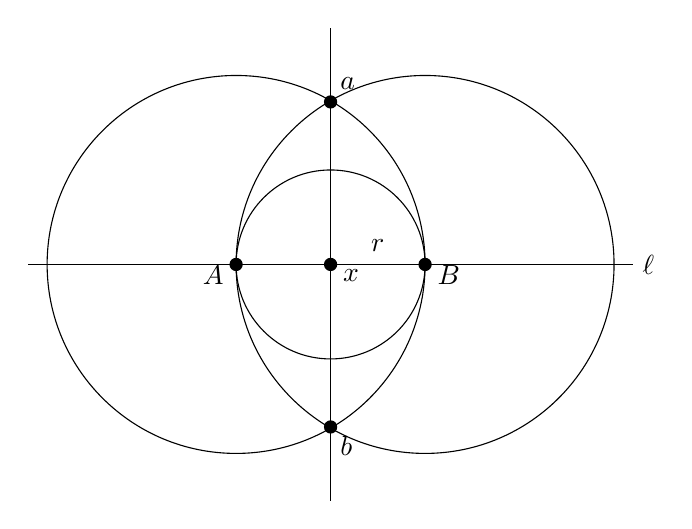
\begin{tikzpicture}[scale=1.2]

% Draw circles
\draw(0,0) circle (1);
\draw (-1,0) circle (2);
\draw (1,0) circle (2);

% Draw horizontal line l
\draw[-] (-3.2,0) -- (3.2,0) node[right] {$\ell$};

% Draw vertical line through intersection
\draw[-] (0,-2.5) -- (0,2.5);

% Points A, x, B,a,b
\fill (-1,0) circle (2pt);
\fill (0,0) circle (2pt);
\fill (1,0) circle (2pt);
\fill (0,-1.72) circle (2pt);
\fill (0,1.72) circle (2pt);

% Labels (slightly below the line)
\node[below=4pt,left=1pt] at (-1,0) {$A$};
\node[below=4pt,right=1pt] at (0,0) {$x$};
\node[below=4pt,right=1pt] at (1,0) {$B$};
\node[above=4pt,right=0pt] at (0,1.8) {$a$};
\node[below=4pt,right=0pt] at (0,-1.8) {$b$};
\node[above=1pt] at (0.5,0) {$r$};

\end{tikzpicture}
\end{center}
\caption{Constructing a line perpendicular to a given line  passing through a point}
\label{fig:perp}
\end{figure}

Given a straight line $\ell$, and a point $x$ on it, let us consider the problem of constructing a line perpendicular to $\ell$ and passing through $x$. We give a construction  in Algorithm \ref{algo:perp}  (See Figure \ref{fig:perp}).
\begin{algorithm}
\begin{algorithmic}[1]
\Procedure{Perpendicular}{$x,\ell$}
\State $c = CIRCLE(x,r)$, where $r$ is a random length
\State $(A,B) = c \cap \ell$  
\State $c_A = CIRCLE(A,2r)$
\State $c_B = CIRCLE(B,2r)$
\State $(a,b) = c_A \cap c_B$
\State $result = LINE(a,b)$
\EndProcedure
\end{algorithmic}
\caption{Constructing a line perpendicular to a given line  passing through a point}
\label{algo:perp}
\end{algorithm}

We have described the algorithmic procedure using some standard primitives. $c = CIRCLE(x,r)$ denotes the construction of a circle $c$  centred at $x$ of radius $r$. $A$ and $B$ are the intersection points of $c$ with $\ell$, denoted in the algorithm as $(A,B) = c \cap \ell$. Similarly, $c_A$ and $c_B$ are circles of radius $2r$ centred at $A$ and $B$ respectively, and $a$ and $b$ are the intersection points of $c_A$ and $c_B$. $LINE(a,b)$ joins $a$ and $b$ and is the $result$.

\begin{exercise}
\begin{enumerate}
\item Convince yourself that the above construction is correct. Use properties of similar triangles.
\item Argue that $LINE(a,b)$ is also the perpendicular bisector of $AB$.
\end{enumerate}
\end{exercise}

\section{Constructing a line parallel to a given line  passing through a point}
\label{sec:parallel}
Given a line $\ell$, and an arbitrary point $x$, consider the problem of construction of a line parallel to $\ell$ passing through $x$. We give a construction  in Algorithm \ref{algo:parallel}  (See Figure \ref{fig:parallel}).

\begin{figure}
\begin{center}
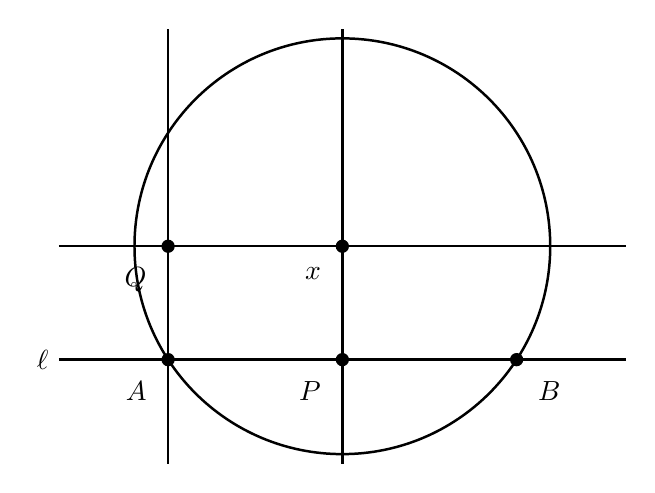
\begin{tikzpicture}[line width=0.9pt, scale=1.2]

% ---- Parameters ----
\pgfmathsetmacro{\R}{2.2}   % circle radius
\pgfmathsetmacro{\h}{1.2}   % vertical offset from center to line \ell (positive)
\pgfmathsetmacro{\dx}{sqrt(\R*\R - \h*\h)} % half-chord length on \ell
\pgfmathsetmacro{\sx}{1.4}  % x-position of side guide lines (cosmetic)

% ---- Geometry ----
\coordinate (X) at (0,0);            % center of circle and label x
\coordinate (A) at (-\dx,-\h);       % left intersection with \ell
\coordinate (B) at ( \dx,-\h);       % right intersection with \ell
\coordinate (P) at (0,-\h);          % point on \ell vertically below x
\coordinate (Q) at (-\dx,0); 

% ---- Circle centered at x ----
\draw (X) circle (\R);

% ---- Horizontal lines: top through x, bottom \ell ----
\draw (-3,0) -- (3,0);                % top line through center
\draw (-3,-\h) -- (3,-\h);            % bottom line \ell
\node[left] at (-3,-\h) {$\ell$};

% ---- Vertical guides (left, center, right) ----
\draw (-\dx,-2.3) -- (-\dx,2.3);
\draw (0,-2.3) -- (0,2.3);
%\draw (\dx,-2.3) -- (\dx,2.3);

% ---- Points ----
\fill (A) circle (2pt);
\fill (B) circle (2pt);
\fill (P) circle (2pt);
\fill (X) circle (2pt);
\fill (Q) circle (2pt);

% ---- Labels (offset so they’re not on the lines) ----
\node[below left=4pt] at (X) {$x$};
\node[below left=4pt]  at (A) {$A$};
\node[below left=4pt]       at (P) {$P$};
\node[below left=4pt]       at (Q) {$Q$};
\node[below right=4pt] at (B) {$B$};

\end{tikzpicture}
\end{center}
\caption{Constructing a line parallel to a given line  passing through a point}
\label{fig:parallel}
\end{figure}

\begin{algorithm}
\begin{algorithmic}[1]
\Procedure{Parallel}{$x,\ell$}
\State $c = CIRCLE(x,r)$, where $r$ is a random length
\State $(A,B) = c \cap \ell$  
\State Construct $p$, the perpendicular bisector of $AB$ using Algorithm \ref{algo:perp}. Argue that $p$ passes through $x$.
\State $P = p \cap \ell$
\State Construct $q$, a perpendicular to $\ell$ passing through $A$ using Algorithm \ref{algo:perp}.
\State Construct $s$, a perpendicular to $p$ passing through $x$ using Algorithm \ref{algo:perp}.
\State $Q = q \cap s$
\State $result = LINE(Q,x)$
\EndProcedure
\end{algorithmic}
\caption{Constructing a line parallel to a given line  passing through a point}
\label{algo:parallel}
\end{algorithm}

Note that in steps 4,6 and 7 of the algorithm, we have used the procedure of Algorithm \ref{algo:perp}. We will routinely use a previously defined algorithm as a primitive to define a new algorithm.
\section{Constructibility and the compass equivalence theorem}

The above two sections give us several examples of construction of points, lines, line segments and circles. The informal definition of {\em constructibility} is as follows.  Given points are by definition constructible. A line joining two constructible points is constructible. So is the circle centred on one constructible point passing through another constructible point. A point is constructible if it is an intersection of constructible lines and circles.

The compass advocated by the Greek philosopher \href{https://en.wikipedia.org/wiki/Plato}{Plato} in these constructions is a {\em collapsing compass}, i.e., a compass that ``collapses'' whenever it is lifted from a page, so that it may not be directly used to transfer distances unlike in a modern fixable aperture compass. Note that nowhere in Sections \ref{sec:perp} and \ref{sec:parallel} have we transferred distances using a fixed size compass lifted from the page.

This is however not a limitation as the following construction shows.

\begin{theorem}
A collapsing compass can be used to transfer a given length to an arbitrary given point on a given line. That is, given an arbitrary length $\overline{AB}$, a line $\ell$ and a point $P$ on it, it is possible to construct using a collapsing compass a point $Q$ on $\ell$ such that $\overline{PQ} = \overline{AB}$.
\end{theorem}
\begin{proof}
\begin{figure}
\begin{center}
\includegraphics[width=0.5\textwidth]{rulercompass/no-collapse.png}

\end{center}
\caption{A compass-equivalence construction}
\label{fig:equiv}
\end{figure}

\begin{algorithm}
\begin{algorithmic}[1]
\Procedure{compass-equivalence}{$A$,$B$,$\ell$,$P$}
\State $c = CIRCLE(A,B)$; note that $\overline{AB} = d$
\State Construct $p$, the line parallel to $\ell$ passing through  $A$ using Algorithm \ref{algo:parallel}
\State $R = c \cap p$
\State $q = LINE(A,P)$
\State Construct $s$, the line parallel to $q$ passing through  $R$ using Algorithm \ref{algo:parallel}
\State $Q = s \cap \ell$
\State $\overline{PQ}$ is the result on $\ell$
\EndProcedure
\end{algorithmic}
\caption{A compass-equivalence construction}
\label{algo:equiv}
\end{algorithm}

\begin{exercise}
Convince yourself that $\overline{PQ} = \overline{AB}$.
\end{exercise}
\end{proof}

The above is different from the original construction and proof of correctness as given by Euclid in his Book of Elements. Interested readers may study a modern version of the original construction \href{https://en.wikipedia.org/wiki/Compass\_equivalence\_theorem}{here}.

\section{Rational numbers are constructible}

\begin{figure}
\begin{center}
\includegraphics[width=0.5\textwidth]{rulercompass/add.png}
\caption{Construction of $a+b$.}
\label{fig:add}
\end{center}
\end{figure}

\begin{figure}
\begin{center}
\includegraphics[width=0.5\textwidth]{rulercompass/sub.png}
\caption{Construction of $a-b$.}
\label{fig:sub}
\end{center}
\end{figure}

%\begin{figure}
%\begin{center}
%\includegraphics[width=0.5\textwidth]{rulercompass/mult.png}
%\caption{Construction of $ab$ given $a$ and $b$.}
%\label{fig:mult}
%\end{center}
%\end{figure}
%
%\begin{figure}
%\begin{center}
%\includegraphics[width=0.5\textwidth]{rulercompass/div.png}
%\caption{Construction of $a/b$ given $a$ and $b$.}
%\label{fig:div}
%\end{center}
%\end{figure}

% Multiplication: OA = a, OU = 1, OB = b, OX = ab.
\begin{figure}
\begin{center}
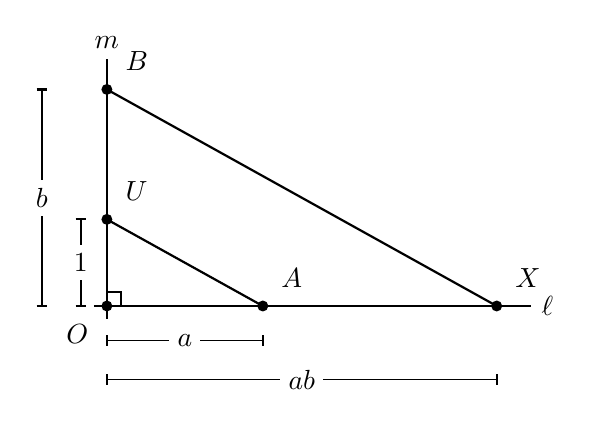
\begin{tikzpicture}[scale=1.1, line width=0.8pt]
    % Illustrative lengths: a = 1.8, b = 2.5.
    \coordinate (O) at (0,0);
    \coordinate (U) at (0,1);
    \coordinate (B) at (0,2.5);
    \coordinate (A) at (1.8,0);
    \coordinate (X) at (4.5,0);

    % Perpendicular lines through O.
    \draw (-0.15,0) -- (4.9,0) node[right] {$\ell$};
    \draw (0,-0.15) -- (0,2.85) node[above] {$m$};

    % AU and the parallel through B.
    \draw (U) -- (A);
    \draw (B) -- (X);

    % Right-angle mark.
    \draw (0,0.16) -- (0.16,0.16) -- (0.16,0);

    % Points and their auxiliary names.
    \foreach \P in {O,U,B,A,X}
        \fill (\P) circle (1.8pt);
    \node[below left=3pt] at (O) {$O$};
    \node[above right=3pt] at (U) {$U$};
    \node[above right=3pt] at (B) {$B$};
    \node[above right=3pt] at (A) {$A$};
    \node[above right=3pt] at (X) {$X$};

    % Vertical length markings.
    \draw[line width=0.5pt]
        (-0.30,0) -- (-0.30,1)
        node[midway,fill=white,inner sep=3pt] {$1$};
    \draw (-0.36,0) -- (-0.24,0);
    \draw (-0.36,1) -- (-0.24,1);

    \draw[line width=0.5pt]
        (-0.75,0) -- (-0.75,2.5)
        node[midway,fill=white,inner sep=3pt] {$b$};
    \draw (-0.81,0) -- (-0.69,0);
    \draw (-0.81,2.5) -- (-0.69,2.5);

    % Horizontal length markings.
    \draw[line width=0.5pt]
        (0,-0.40) -- (1.8,-0.40)
        node[midway,fill=white,inner sep=3pt] {$a$};
    \draw (0,-0.46) -- (0,-0.34);
    \draw (1.8,-0.46) -- (1.8,-0.34);

    \draw[line width=0.5pt]
        (0,-0.85) -- (4.5,-0.85)
        node[midway,fill=white,inner sep=3pt] {$ab$};
    \draw (0,-0.91) -- (0,-0.79);
    \draw (4.5,-0.91) -- (4.5,-0.79);
\end{tikzpicture}
\end{center}
\caption{Construction of $ab$ given $a$ and $b$.
Join $A$ to $U$ and draw the parallel through $B$,
meeting $\ell$ at $X$. Then $\overline{OX}=ab$.}
\label{fig:mult}
\end{figure}


% Division: OA = a, OB = b, OU = 1, OX = a/b.
\begin{figure}
\begin{center}
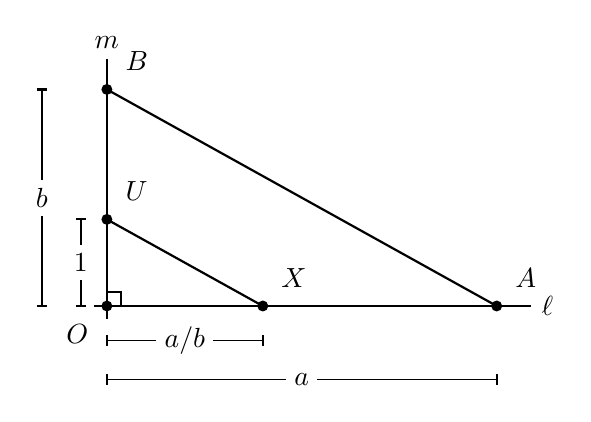
\begin{tikzpicture}[scale=1.1, line width=0.8pt]
    % Illustrative lengths: a = 4.5, b = 2.5.
    \coordinate (O) at (0,0);
    \coordinate (U) at (0,1);
    \coordinate (B) at (0,2.5);
    \coordinate (X) at (1.8,0);
    \coordinate (A) at (4.5,0);

    % Perpendicular lines through O.
    \draw (-0.15,0) -- (4.9,0) node[right] {$\ell$};
    \draw (0,-0.15) -- (0,2.85) node[above] {$m$};

    % AB and the parallel through U.
    \draw (B) -- (A);
    \draw (U) -- (X);

    % Right-angle mark.
    \draw (0,0.16) -- (0.16,0.16) -- (0.16,0);

    % Points and their auxiliary names.
    \foreach \P in {O,U,B,A,X}
        \fill (\P) circle (1.8pt);
    \node[below left=3pt] at (O) {$O$};
    \node[above right=3pt] at (U) {$U$};
    \node[above right=3pt] at (B) {$B$};
    \node[above right=3pt] at (X) {$X$};
    \node[above right=3pt] at (A) {$A$};

    % Vertical length markings.
    \draw[line width=0.5pt]
        (-0.30,0) -- (-0.30,1)
        node[midway,fill=white,inner sep=3pt] {$1$};
    \draw (-0.36,0) -- (-0.24,0);
    \draw (-0.36,1) -- (-0.24,1);

    \draw[line width=0.5pt]
        (-0.75,0) -- (-0.75,2.5)
        node[midway,fill=white,inner sep=3pt] {$b$};
    \draw (-0.81,0) -- (-0.69,0);
    \draw (-0.81,2.5) -- (-0.69,2.5);

    % Horizontal length markings.
    \draw[line width=0.5pt]
        (0,-0.40) -- (1.8,-0.40)
        node[midway,fill=white,inner sep=3pt] {$a/b$};
    \draw (0,-0.46) -- (0,-0.34);
    \draw (1.8,-0.46) -- (1.8,-0.34);

    \draw[line width=0.5pt]
        (0,-0.85) -- (4.5,-0.85)
        node[midway,fill=white,inner sep=3pt] {$a$};
    \draw (0,-0.91) -- (0,-0.79);
    \draw (4.5,-0.91) -- (4.5,-0.79);
\end{tikzpicture}
\end{center}
\caption{Construction of $a/b$ given $a$ and $b$, $b>0$.
Join $A$ to $B$ and draw the parallel through $U$,
meeting $\ell$ at $X$. Then $\overline{OX}=a/b$.}
\label{fig:div}
\end{figure}


First, we can consider any given length as 1, measure it using a non-collapsing compass -- which we just proved is equivalent to a collapsing compass -- and add it to any point on a given line by marking it off with the compass. We can similarly subtract. The operations $S(n)$ and $P(n)$ are thus realisable using ruler and compass. Consequently, the elements of the set $\Z$ are constructible. In Figures \ref{fig:add} and \ref{fig:sub} we give the direct constructions for $a+b$ and $a-b$.

Given integers $a$ and $b$ as line segments, we can also construct rational number $ab$ and $a/b$ directly using similar triangles. The construction of Figure \ref{fig:mult} involves marking off the lengths $a$ and $b$ in two perpendicular segments from $O$, constructing the unit length in the direction of $b$, and constructing a line parallel to the line $\overline{a1}$ through $a$ or $b$. The intercept of the parallel line in the direction of $a$ then marks  the length $ab$ by similarity of the triangles. We can similarly construct $a/b$ as depicted in Figure \ref{fig:div}. Rational numbers are thus constructible.  See the following Algorithms:

\begin{algorithm}
\begin{algorithmic}[1]
\Procedure{Multiply}{$a,b$}
\State Choose a horizontal line $\ell$ and a point $O$ on it
\State Construct $m$, the perpendicular to $\ell$ passing
       through $O$ using Algorithm \ref{algo:perp}
\State $c_a = CIRCLE(O,a)$
\State $A = c_a \cap \ell$, choosing the intersection
       to the right of $O$
\State $c_1 = CIRCLE(O,1)$
\State $U = c_1 \cap m$, choosing the intersection
       above $O$
\State $c_b = CIRCLE(O,b)$
\State $B = c_b \cap m$, choosing the intersection
       above $O$
\State $p = LINE(A,U)$
\State Construct $q$, the line parallel to $p$ passing
       through $B$ using Algorithm \ref{algo:parallel};
       if $B=U$, take $q=p$
\State $X = q \cap \ell$
\State $\overline{OX}$ is the result on $\ell$
\EndProcedure
\end{algorithmic}
\caption{Constructing $ab$ given $a$ and $b$}
\label{algo:mult}
\end{algorithm}

\begin{algorithm}
\begin{algorithmic}[1]
\Procedure{Divide}{$a,b$}
\State Choose a horizontal line $\ell$ and a point $O$ on it
\State Construct $m$, the perpendicular to $\ell$ passing
       through $O$ using Algorithm \ref{algo:perp}
\State $c_a = CIRCLE(O,a)$
\State $A = c_a \cap \ell$, choosing the intersection
       to the right of $O$
\State $c_b = CIRCLE(O,b)$
\State $B = c_b \cap m$, choosing the intersection
       above $O$
\State $c_1 = CIRCLE(O,1)$
\State $U = c_1 \cap m$, choosing the intersection
       above $O$
\State $p = LINE(A,B)$
\State Construct $q$, the line parallel to $p$ passing
       through $U$ using Algorithm \ref{algo:parallel};
       if $U=B$, take $q=p$
\State $X = q \cap \ell$
\State $\overline{OX}$ is the result on $\ell$
\EndProcedure
\end{algorithmic}
\caption{Constructing $a/b$ given $a$ and $b$, $b>0$}
\label{algo:div}
\end{algorithm}

\begin{exercise}
\begin{enumerate}
\item Describe a ruler and compass procedure for multiplication using repeated additions.
\item Describe a ruler and compass procedure for division (computing quotient and remainder) using repeated subtractions.
\end{enumerate}
\end{exercise}



\section{Euclid's GCD using ruler and compass}
\label{sec:gcd}
GCD of two integers $a > 0$, $b \geq 0$ is defined as the largest integer $d, d > 0$ that divides both $a$ and $b$. Consider the following algorithm for computing the GCD:
        \[
                gcd(a,b)
                 = \left\{      \begin{array}{ll}
                                a       &                     \mbox{if $b = 0$} \\
                                a       &                     \mbox{if $a = b$} \\
                                gcd(a-b,b)      &       \mbox{if $a > b$} \\
                                gcd(a,b-a)      &       \mbox{if $b > a$}
                                \end{array}
                        \right.
        \]
\begin{exercise}
\begin{enumerate}
\item        Convince yourself that the above algorithmic specification (rule) is correct for computing GCD. Carry out the pencil and paper computation using the  above algorithm for some  special cases.
\item         Describe the procedure for executing the algorithm using ruler and compass.
\end{enumerate}
\end{exercise}

The algorithm described above is from Euclid's Elements. You can find a description of it \href{https://en.wikipedia.org/wiki/Euclidean_algorithm}{here}. This is also considered to be the oldest non-trivial algorithm in common use.

Now that we have defined our first computational model, several questions arise. What are the full powers of the model? What are the other things that can be constructed? What are the limits of the model, and are there easily defied concepts that are not constructible? Can there be other computational models more powerful than ruler and compass?  These are the kind of questions we interrogate every computational model with. We will revisit some of these questions in the latter chapters.

\begin{exercise}
\label{exer:squarerootof2}
 Try to construct $\sqrt{2}$ using ruler and compass. (Hint: Use the Pythagoras theorem 
  on a right triangle with sides $1, 1$.) Argue why this length is constructible.
  \label{exer:sqrt2}
\end{exercise}


\section*{Problems}

\begin{enumerate}
  %\setcounter{enumi}{4}

  \item Construct, using ruler and compass, the perpendicular bisector of a line segment $AB$. 
  Show that any point $P$ on the perpendicular bisector is equidistant from $A$ and $B$.

  \item Given a triangle $ABC$, construct the three medians using ruler and compass. 
  Argue that they intersect at a single point (the centroid).  

  \item Using Algorithm~3 (perpendicular construction), describe step by step how to construct 
  the altitude from a vertex of a triangle. Illustrate your steps with a figure.

  \item Given a line $\ell$ and an external point $P$, use Algorithm~4 (parallel construction) 
  to draw the line parallel to $\ell$ through $P$. Prove that the two lines do not intersect.

  \item Show that the compass-equivalence construction (Algorithm~5) indeed allows one to 
  transfer a given length $AB$ to an arbitrary point $P$ on a line $\ell$. 
  Verify your construction with a worked example.

  \item Describe a ruler and compass procedure for multiplication of two integers $a, b$ 
  using repeated additions. Demonstrate the construction for $a=3, b=4$.

  \item Similarly, describe a ruler and compass procedure for division using repeated subtractions. 
  Apply your method to compute the quotient and remainder when dividing a segment of length $11$ 
  into parts of length $3$.

  \item Using constructions based on similar triangles, show step by step how to obtain 
  the product $ab$ given line segments $a$ and $b$.

  \item Construct the rational number $\tfrac{3}{5}$ on a line, starting with a unit segment. 
  Explain each step of your construction.

  \item Apply Euclid’s GCD algorithm (as given in Section 3.5) to the lengths $a = 21$, $b = 15$, 
  using repeated subtraction with compass and ruler. Show all intermediate steps.

  \item Prove that Euclid’s GCD algorithm terminates in a finite number of steps for all $a, b \in \mathbb{N}$. 
  (Hint: in each step one of the arguments strictly decreases.)

   

\end{enumerate}

